%!TEX TS-program = xelatex
%!TEX encoding = UTF-8 Unicode

\documentclass[12pt]{extarticle}
% extarticle is like article but can handle 8pt, 9pt, 10pt, 11pt, 12pt, 14pt, 17pt, and 20pt text

\def \ititle {Origins of Mind}
 
\def \isubtitle {Lecture 08}
 
\def \iauthor {Stephen A. Butterfill}
\def \iemail{s.butterfill@warwick.ac.uk}
\date{}

%for strikethrough
\usepackage[normalem]{ulem}

\input{$HOME/Documents/submissions/preamble_steve_handout}

%logic symbol \leftmodels
\usepackage{MnSymbol}

%\bibpunct{}{}{,}{s}{}{,}  %use superscript TICS style bib
%remove hanging indent for TICS style bib
%TODO doesnt work
\setlength{\bibhang}{0em}
%\setlength{\bibsep}{0.5em}


%itemize bullet should be dash
\renewcommand{\labelitemi}{$-$}

\begin{document}

\raggedcolumns

\begin{multicols*}{3}

\setlength\footnotesep{1em}


\bibliographystyle{newapa} %apalike

%\maketitle
%\tableofcontents




%--------------- 
%--- start paste
\def \ititle {Logic I}
 
\def \isubtitle {Fast Lecture 07}
 
\begin{center}
 
{\Large
 
\textbf{\ititle}: \isubtitle
 
}
 
 
 
\iemail %
 
\end{center}
 
Readings refer to sections of the course textbook, \emph{Language, Proof and Logic}.
 
 
 
\section{Every Time I Go to the Dentist Someone Dies}
 
\emph{Reading:} §11.2
 
∀t (
 
\hspace{5mm} (Time(t) ∧ ToDentist(a,t) )
 
\hspace{5mm} →
 
\hspace{5mm} ∃x ( Person(x) ∧ TimeOfDeath(x,t) )
 
)
 
\vfill
\columnbreak

\section{Truth-functional completeness}
 
\emph{Reading:} §7.4
 
‘A set of truth-functors is said to be \emph{expressively adequate} (or sometimes \emph{functionally complete}) iff, for every truth-function whatever, there is a formula containing only those truth-functors which express that truth-function, i.e. which has as its truth-table the truth-table specifying that function.’ (Bostock, \emph{Intermediate Logic} p. 45)
 
Illustration of the proof that $\{$¬, ∧, ∨$\}$ is truth-functionally complete:
 
\begin{center}
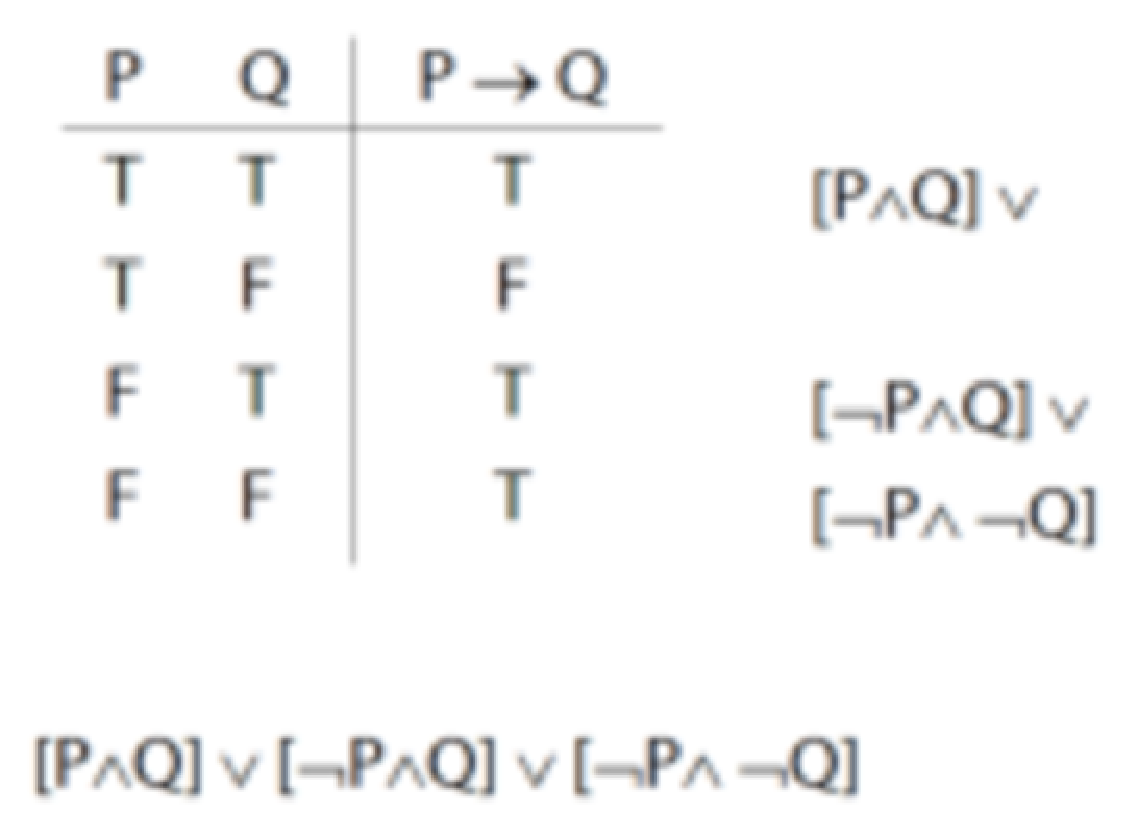
\includegraphics[scale=0.3]{img/unit_430_fig2.pdf}
\end{center}
\emph{Exercise} assuming $\{$¬,∨,∧$\}$ is truth-functionally complete, show that $\{$¬,∨$\}$ is.
 



\section{Proofs about Proofs}
 
\begin{minipage}{\columnwidth}
 
\textbf{If A $\vdash$ B then $\vdash$ A→B}
 
Proof Given a proof for A $\vdash$ B …
 
\begin{center}
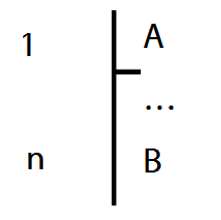
\includegraphics[scale=0.3]{img/unit_440_a.png}
\end{center}
… we can turn it into a proof for $\vdash$ A→B:
 
\begin{center}
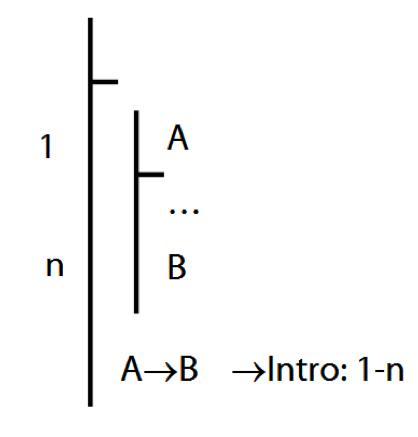
\includegraphics[scale=0.3]{img/unit_440_b.png}
\end{center}
\end{minipage}
 
\textbf{If $\vdash$ A→B then A $\vdash$ B}
 
\begin{minipage}{\columnwidth}
 
\textbf{If A $\vdash$ B then A $\vdash$ ¬¬B}
 
Proof:
 
\begin{center}
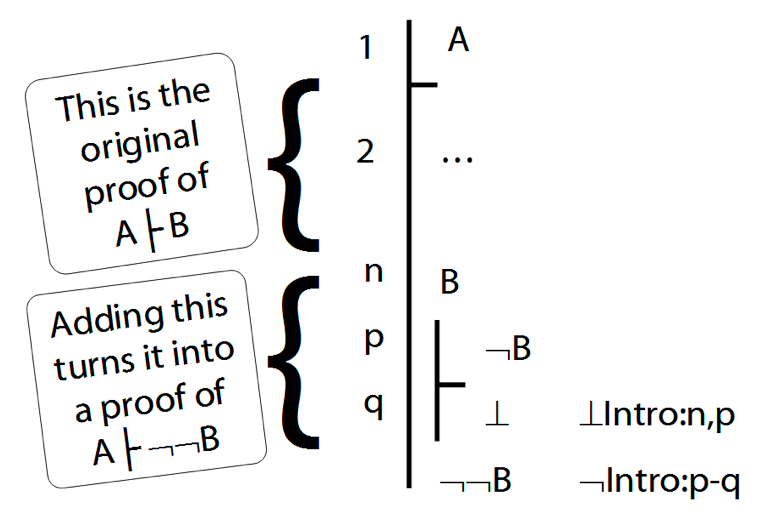
\includegraphics[scale=0.3]{img/unit_440_c.png}
\end{center}
\end{minipage}
 
\textbf{If A $\vdash$ C then A $\vdash$ B→C}
 
\textbf{If A $\vdash$ B and A $\vdash$ ¬C then A $\vdash$ ¬(B→C)}
 
 
 
\section{The Soundness Property and the Fubar Rules (fast)}
 
\emph{Reading:} §8.3
 
\begin{center}
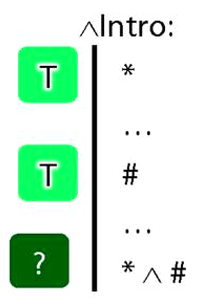
\includegraphics[scale=0.3]{img/unit_346_and.png}
\end{center}
\begin{center}
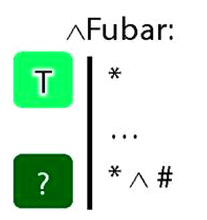
\includegraphics[scale=0.3]{img/unit_346_fubar.png}
\end{center}
 
 
\section{Proof of the Soundness Theorem}
 
\emph{Reading:} §8.3
 
\begin{minipage}{\columnwidth}
 
\textbf{Illustration of soundness proof: ∨Intro}
 
\begin{center}
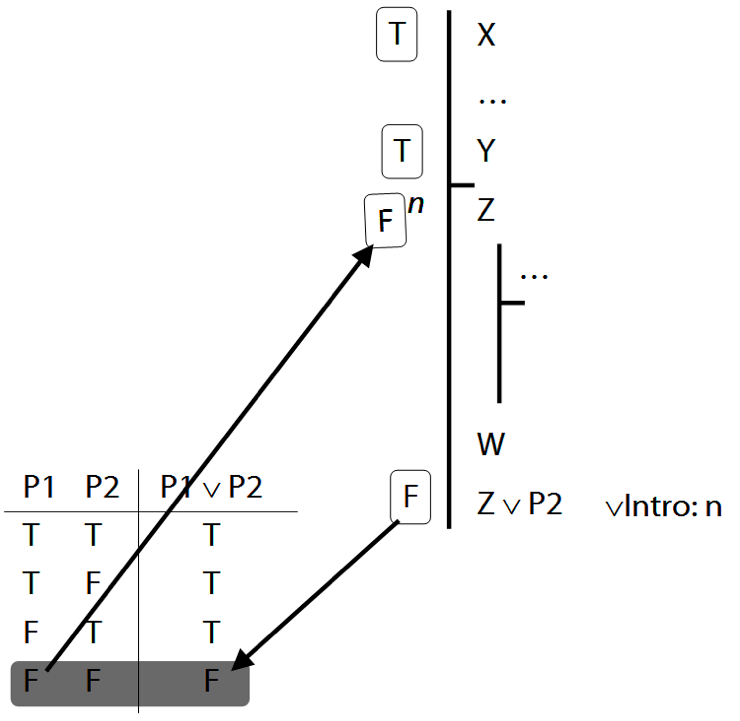
\includegraphics[scale=0.3]{img/soundness_or.png}
\end{center}
\end{minipage}
 
\emph{Useful Observation about any argument that ends with ∨Intro.} Suppose this argument is not valid, i.e. the premises are true and the conclusion false. Then Z must be false. So Z cannot be a premise.  But the argument from the premises to Z (line n) is not a valid argument. So there is a shorter proof which is not valid.
 
\emph{Stipulation}: when I say that \emph{a proof is not valid}, I mean that the last step of the proof is not a logical consequence of the premises (including premises of any open subproofs).
 
\begin{minipage}{\columnwidth}
 
\textbf{Illustration of soundness proof: ¬Intro}
 
\begin{center}
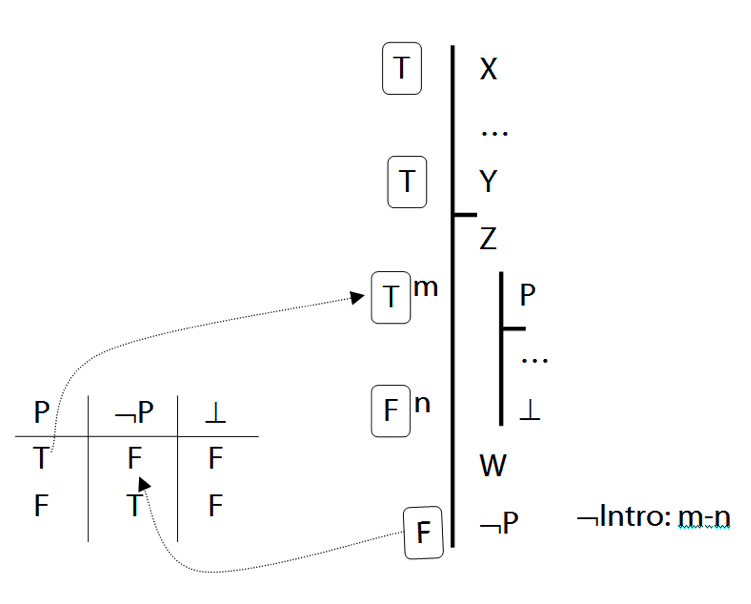
\includegraphics[scale=0.3]{img/soundness_not.png}
\end{center}
\end{minipage}
 
\begin{minipage}{\columnwidth}
 
\textbf{How to prove soundness? Outline}
 
Step 1: show that each rule has this property:
 
\hspace{5mm} Where the last step in a proof involves that rule, if proof is not valid then there is a shorter proof which is not valid.
 
Step 2: Suppose (for a contradiction) that some Fitch proofs are not valid. Select one of the shortest invalid proofs. The last step must involve one of the Fitch rules. Whichever rule it involves, we know that there must be a shorter proof which is not valid. This contradicts the fact that the selected proof is a shortest invalid proof.
 
\end{minipage}
 
 
 
\section{The Essence of the Completeness Theorem}
 
\emph{Reading:} §8.3
 
\begin{center}
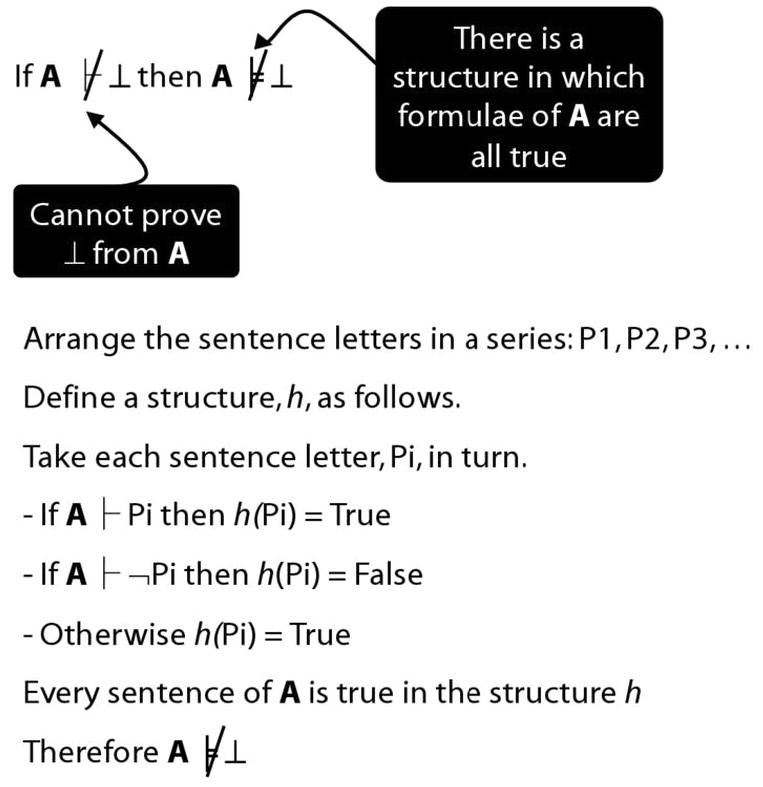
\includegraphics[scale=0.3]{img/unit_450.png}
\end{center}
 
 
 
 
\section{Lemma for the Completeness Theorem}
 
\emph{Reading:} §8.3
 
 
If for every sentence letter, P, either A $\vdash$ P or A $\vdash$ ¬P, then for every formula, X, either A $\vdash$ X or A $\vdash$ ¬X.
 
Proof
 
\textbf{Step a.} Suppose (for a contradiction) that there are formulae, X, such that A $\nvdash$ X and A $\nvdash$ ¬X. Take a shortest such formula, call it Y.
 
\textbf{Step b.} This formula, Y, must have one of the following forms: ¬P, P∨Q, P∧Q, P→Q, P↔Q, $\bot$
 
\textbf{Step c.} We can show that whichever form X has, either A $\vdash$ Y and A $\vdash$ ¬Y.
 
Case 1: X is P→Q. Then since P and Q are shorter than X, either:
 
\hspace{5mm} (i) A $\vdash$ P and A $\vdash$ ¬Q
 
\hspace{5mm} or
 
\hspace{5mm} (ii) A $\vdash$ ¬P
 
\hspace{5mm} or
 
\hspace{5mm} (iii) A $\vdash$ Q
 
\hspace{5mm} If (i), A $\vdash$ ¬(P→Q), that is, A $\vdash$ ¬X.
 
\hspace{5mm} If (ii), A $\vdash$ P→Q, that is, A $\vdash$ ¬X.
 
\hspace{5mm} If (iii), A $\vdash$ P→Q, that is, A $\vdash$ ¬X.
 
\hspace{5mm} (Here we use the last two Proofs about Proofs, see earlier)
 
Case 2: X is ¬P.
 
\hspace{5mm} Then since P is shorter, A $\vdash$ P or A $\vdash$ ¬P.
 
\hspace{5mm} If A $\vdash$ P then A $\vdash$ ¬¬P so A $\vdash$ ¬X which would contradict our assumption. This is shown in the proofs about proofs above.
 
\hspace{5mm} If A $\vdash$ ¬P then A $\vdash$ X (because X is ¬P), which would contradict our assumption.
 
Case 3: …
 
\textbf{Step d.} The demonstration in Step c contradicts our assumption, so we can conclude that it is false. That is, either A $\vdash$ X and A $\vdash$ ¬X for every formula X.
 
 
 
\section{Proof of the Completeness Theorem}
 
\emph{Reading:} §8.3, §17.2
 
\begin{center}
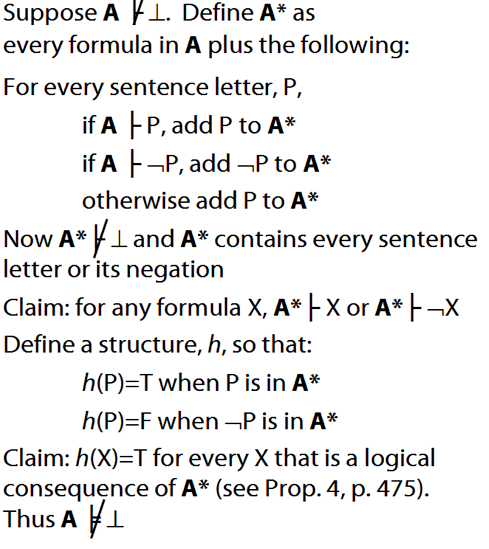
\includegraphics[scale=0.35]{img/unit_455_completeness.png}
\end{center}
 
 
\section{More Records Than the KGB}
 
\emph{Reading:} §14.1, §14.3
 
 
 
\section{The End Is Near}
 
\emph{Reading:} §14.3
 
%--- end paste
%--------------- 
 

\end{multicols*}

\end{document}